%! TEX root = 0-main.tex
\chapter{Causality}
Consider the schwarzschild metric as \(r\to r_s\). The gravitational redshift of a photon at \(r_e\) can be found
\[\frac{\omega(r)}{\omega(r_e)} = \sqrt{\frac{g_{tt}(r_e)}{g_{tt}(r)}}\]
as \(r\to r_s\) we find that \(\omega(r)/\omega(r_e)\to \infty\), or equivalently, if the photon is emitted at \(r\) and detected at \(r_d\), we find \(\omega(r_d)/\omega(r)\to0\), or that the light emitted at the event horizon is redshifted to zero always.

If we consider the radial lightcones
\[\d{s}^2 = 0=-\left(1-\frac{r_s}{r}\right)\d{t}^2+ \left(1-\frac{r}{r_s}\right)^{-1}\d{r}^2\]
\[\d{t} = \pm \frac{r}{r-r_s}\d{r}\]
for \(+\), we have the outward lightcone, as an increase in \(\d{t}\) leads to an increase in \(\d{r}\); for \(-\), we have correspondingly the inward lightcone. 

As \(r\to\infty\), we recover the minkowski light cones. As we approach \(r_s\), the cone gets narrower and narrower, until we reach \(r_s\), and the lightcone collapses, and inside \(r_s\), our coordinates become meaningless

We change our coordinates by
\[\d{\bar t} = \d{t} + \frac{r_s}{r-r_s}\d{r}\]
allowing us rewrite
\[\d{s}^2 = \left(\frac{r-r_s}{r}\right)\left(\d{\bar t}+\d{r}\right)\left(\d{\bar t} - \frac{r+r_s}{r-r_s}\d{r}\right)\]
we then have two lightcones---the incoming light cone
\[\der{\bar t}{r} = -1\]
and the outgoing
\[\der{\bar t}{r} = \frac{r+r_s}{r-r_s}\]
we can then find a family of lightcone solutions, shown in Fig.~\ref{fig:bheh}

\begin{figure}[!htbp]
\begin{center}
	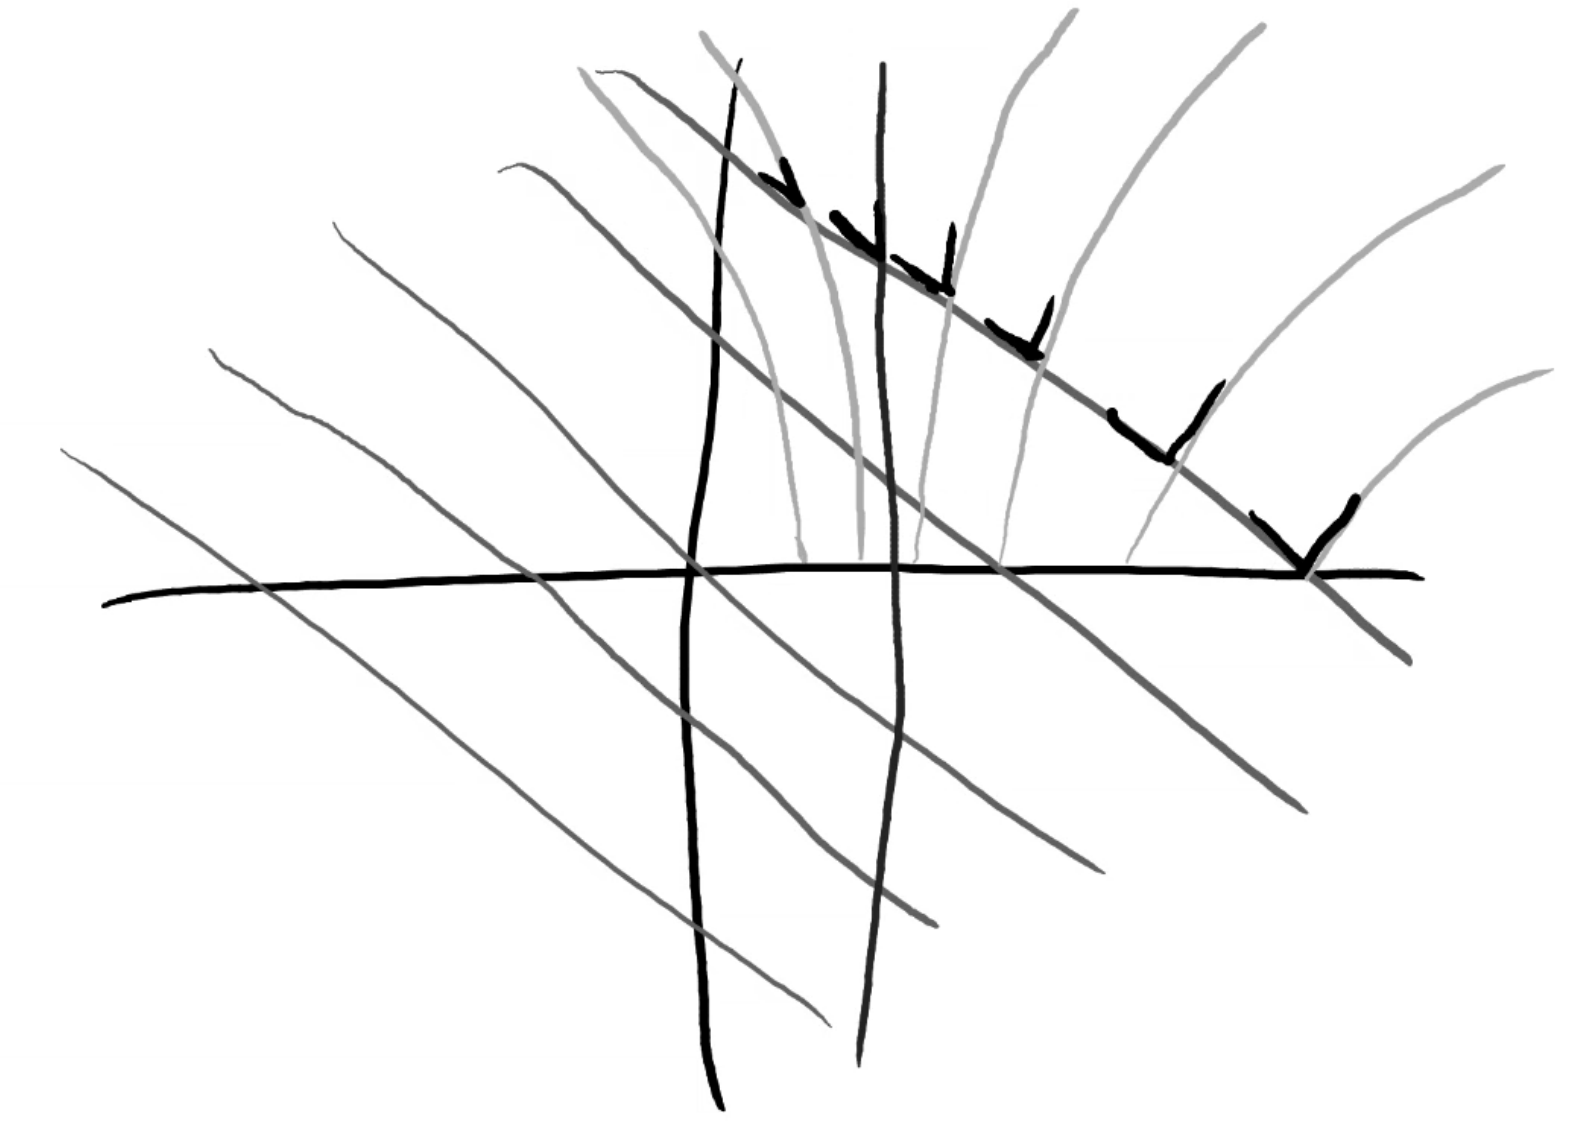
\includegraphics[width = 0.7\textwidth]{Figures/Ch8/bh eh.png}
\end{center}
\caption{Lightcones for Black Hole}\label{fig:bheh}
\end{figure}

We then see that as one goes toward the singularity of the event horizon, the light cones pinch off and tilt toward the singularity, and once the particle passes the event horizon, the particle can no longer escape, as no part of the light cone points outward.

However, this isn't very elucidating in the \(r\) direction at the event horizon; what happens to a photon moving radially outward starting at the event horizon?

\section{Eddington-Finkelstein Coordinates}
Note that we can factor the Schwarzschild metric as
\[\d{s}^2 = -\left(\frac{r-r_s}{r}\right)\left(\d{t}+\frac{r}{r-r_s}\d{r}\right)\left(\d t + \frac{r}{r-r_s}\d{r}\right)+ r^2\d\Omega^2\]
We can refine the coordinates by using
\[\d{v}= = \d{t}+\frac{r}{r-r_s}\d{r}\]
so
\[\d{s}^2 = -\left(\frac{r-r_s}{r}\right)\d{v}^2 - 2\d{v}\d{r} + r^2\d\Omega^2\]

we find radial light rays follow
\[\left(\frac{r-r_s}{r}\right)\d{v}=2\d{r}\]
integrating, we find
\[v=  t + r + r_s\ln\abs{\dfrac{r-r_s}{r}} = \bar t + r\]
\section{Kruskal-Szekeres Coordinates}
Note that there is one more term that seems very evocative of a subsitution. Thus, 
\[\d p = \d t + \frac{r}{r-r_s}\d{r} \qquad\qquad \d q = \d t - \frac{r}{r-r_s}\d{r}\]
so
\[\d{s} = -\left(\frac{r-r_s}{r}\right)\d p\d q + r^2\d \Omega\]
However, notice that
\[\d{(p+q)} = 2\d t \qquad \d{(p-q)} = 2\left(1+\frac{r_s}{r-r_s}\right)\d{r}\]
or
\[p+q = 2t \qquad\qquad p-q = 2r+r_s\log\abs{\dfrac{r-r_s}{r}}\]
we see that for \(r\gg r_s\) the second term vanishes and we recover minkowski space, as we expect.

Changing coordinates once more,
\[P = e^{p/2r_s} \qquad\qquad Q=e^{-q/2r_s}\]
we find
\[\d{s}^2 = -\frac{4r_s}{r}e^{-r/r_s}\sgn(r-r_s)\d{P}\d{Q} + r^2\d\Omega^2\]
Recall that
\[\sgn(x)\equiv \begin{cases}
	-1 & x<0\\
	0 & x = 0\\
	1 & x > 0
\end{cases}\]
This reveals that the only \emph{true} singularity is \(r=0\), while the \(r=r_s\) singularity earlier was due only to a coordinate singularity.

Once again transforming coordinates,
\[V = \frac{1}{2}(P+Q) \qquad\qquad U = \frac{1}{2}(P-Q)\]
we find
\[\d{V}^2 + \d{Q}^2 = \d P\d Q\]
\[\d{V}^2 - \d Q ^2 = \sgn(r-r_s)\d P\d Q\]
so
\begin{equation}
\d{s}^2= -\frac{4r_s}{r}e^{-r/r_s}\left(\d{V}^2+\d{U}^2\right) + r^2\d\Omega^2
\end{equation}
and that radial light rays are given
\[\d{U} = \pm\d{V}\]

however, we note that because \(\d{V}^2-\d{U}^2\) has the signum function in it, we have within the schwarzschild radius that \(V\) and \(U\) switch; that is
\[V(r<r_s) = \frac{1}{2}(P-Q)\qquad \qquad U(r<r_s) = \frac{1}{2}(P+Q)\]
from some algebra, we find
\[V^2+U^2 = \left(1-\frac{r}{r_s}\right)e^{r/r_s}\]
and that outside the event horizon
\[\frac{V}{U} = \frac{P+Q}{P-Q} = \tanh\frac{t}{2r_s}\]
and inside it
\[\frac{V}{U} = \frac{P-Q}{P+Q} = \coth\frac{t}{2r_s}\]
allowing us to write (outside the horizon)
\[V = \left(\frac{r}{r_s}-1\right)^{1/2}e^{r/2r_s}\sinh\frac{t}{2r_s}\]
\[U = \left(\frac{r}{r_s}-1\right)^{1/2}e^{r/2r_s}\cosh\frac{t}{2r_s}\]
and reversed inside the horizon.

Lines of constant \(t\) give radial lines, while \(t=\infty\) corresponds to \(V = \pm U\). Similarly, lines of constant \(r\) give hyperbolae, which face along the \(U\) direction outside \(r_s\), and point along \(V\) inside \(r_s\). At \(r_s\) we have \(V=\pm U\) once again, and at \(r=0\) we obtain the parabolae
\[V = \sqrt{U^2+1}\]
recall the lightcone structure is given \(\d{V} = \pm\d{U}\)

We define the the regions, separated by the event horizon as I through IV going counterclockwise from the +ve U axis. I is the space outside the black hole, II is inside the schwarzschild black hole, while III is a wormhole, and IV is a white hole region.

Note that objects within the \emph{anti-horizon}, the white hole's \(r=2M\) plane, can causally impact region I but cannot be in turn causally affected; this is the opposite of the black hole. Similarly, because of the causal structure, when you cross the horizon, you see all the light that ever passed through the event horizon.

Further, note that due to the causal structure, it is impossible for a massive particle to reach the other side of the wormhole. However, if we take the metric for \(t=0\then V=0\), we find the metric becomes
\[\d{s}^2= \frac{4 r_s^3}{r}e^{-r/r_s}\d{U}^2 + r^2\d\Omega^2\]
further, our slice gives
\[U = \left(\frac{r}{r_s}-1\right)^{1/2} e^{r/2r_s}\]
which upon substitution yields
\[\d{s}^2 = \frac{1}{1-\frac{r_s}{r}}\d{r}+r^2\d\Omega^2\]
Varying \(V\) shows us that the wormhole is ``pinched off'' by intersection with the singularity and separated soon after formation; the wormhole is not static but has a dynamic evolution.
\[\d{s}^2 = \frac{1}{1-\frac{r_s}{r}\left(1-V_0 e^{-r/r_s}\right)}\d{r}^2+r^2\d\Omega^2\]
The timescale wher the wormhole is open is on the order of \(r_s=2M\)
